%%
%% FIT2026 投稿用原稿
%% カテゴリ: D-2 情報基礎とアクセス技術(IFAT)
%%
\documentclass[submit,techrep,noauthor]{ipsj}

\usepackage[dvipdfmx]{graphicx}
\usepackage{latexsym}
\usepackage{url}
\usepackage{tikz}
\usepackage{pgfplots}
\pgfplotsset{compat=1.18}
\usetikzlibrary{shapes.geometric, arrows.meta, positioning}

\def\Underline{\setbox0\hbox\bgroup\let\\\endUnderline}
\def\endUnderline{\vphantom{y}\egroup\smash{\underline{\box0}}\\}
\def\|{\verb|}

\begin{document}

\title{XPathGenie: LLM駆動による自動XPath生成\\
——マルチページ検証と二段階精緻化}

\affiliate{BS}{bon soleil}

\author{川嶋 力}{Tsutomu Kawashima}{BS}

\begin{abstract}
本稿では,生のURLから再利用可能なXPath式の生成を自動化するシステムXPathGenieを提案する.
本システムはHTMLの構造的圧縮(約97\%削減),LLMに基づく推論,マルチページ検証,
および二段階精緻化を組み合わせ,AIの呼び出しをサイトあたり一度に限定することで
以降の抽出コストをゼロとする.
サイトあたりのエンドツーエンド所要時間は約20分であり,
手作業によるXPath記述の5--6時間から大幅に短縮される.
23の医療系求人サイトでの手動評価ではセマンティック精度95.0\%,
SWDEベンチマーク(22サイト)ではラベル付き訓練データなしの
ゼロショット設定で検出フィールドF1=0.689を達成した.
\end{abstract}

\maketitle

%% =============================================
\section{はじめに}

Webサイトからの構造化データ抽出は,競合情報分析,求人情報集約,
価格監視をはじめとする多様なデータ駆動型アプリケーションの基盤技術である.
大半の抽出パイプラインの中核にはXPath——HTML/XML文書のDOM(Document Object Model:
文書の要素構造を木構造で表現するモデル)からノードを選択するためのクエリ言語——が
位置している.例えば\texttt{//span[@class='price']}は「class属性がpriceである
span要素をすべて取得する」という指示となる.しかし,その記述は依然として
手作業に大きく依存している.

この領域の課題は三つに集約される.
第一に\textbf{時間的コスト}である.単一のWebサイトに対して信頼性の高いXPath
マッピングを構築するには,ページの精査,式の記述,エッジケースへの対応,
およびクロスページ検証を含め通常数時間の専門的作業を要する.
第二に\textbf{暗黙知への依存}である.実効的なXPath構築には一般的なHTMLパターン
(定義リスト,テーブルレイアウト,ネストされたコンテナ)やサイト固有の特異性に
関する理解が必要であるが,この知識の体系化は困難である.
第三に\textbf{スケーラビリティ}である.サイトの構造変更のたびに既存のXPathは
無効となり,ポートフォリオ規模に比例した継続的保守が必要となる.

本研究は人間の判断を排除するのではなく,自動化パイプライン内における限定的かつ
構造化された介入として再配置することを目指す.XPathGenieはXPath生成を
構造的に圧縮されたHTML上でのLLM推論問題として再定式化し,決定論的な検証および
精緻化段階で補強する.中核的な設計思想は「AI Once, DOM Forever」——AIの呼び出しを
初期マッピング発見のただ一度に限定し,以降のすべての処理を追加AI費用ゼロの
DOM操作のみで実行する——という点にある.

本研究はLLMをランタイムの抽出エンジンではなく設計時のXPathコンパイラとして
位置づけ直すことで,抽出コストモデルを根本的に変革する.
本論文の貢献は以下の三点である.
(1) LLM呼び出しをサイトあたり定数回に限定し,抽出対象ページ数$n$に依存しない
$O(1)$コストで以降の抽出を決定論的DOM操作のみで実行する
「AI Once, DOM Forever」アーキテクチャ,
(2) XPath構築に必要なDOM階層を保持しつつ約97\%のサイズ削減を達成する
構造保持型HTML圧縮(中間表現),
(3) 機械的絞り込み(AIコストゼロ)とAI再推論を組み合わせた
検証駆動型二段階精緻化フレームワーク.
これらを2言語・15以上のドメインにまたがる62サイト規模で多面的に評価した.

%% =============================================
\section{関連研究}

Webデータの自動抽出は広範に研究されている.
ラッパー帰納システム\cite{kushmerick1997,dalvi2011}はラベル付き事例から
抽出ルールを学習するが,ターゲットスキーマごとに訓練データを必要とする.
MarkupLM\cite{li2022}やDOM-LM\cite{deng2022}等のHTML対応言語モデルは
DOM構造の理解を深めたが,ファインチューニングが前提である.
ScrapeGraphAI\cite{perini2024}はグラフベースのパイプラインでLLMを制御するが,
抽出時にページごとにLLMを呼び出すためコストが線形に増加する.

XPathGenieに最も近い関連研究として,
XPath Agent\cite{xpathagent2024}は二段階LLMパイプラインによるXPath生成を,
AXE\cite{axe2026}は97.9\%のDOM枝刈りと0.6Bパラメータモデルにより
SWDEベンチマークでF1 88.1\%を報告している.

XPathGenieとこれらのシステムの主要な差異は以下の通りである.
(1) \textbf{生成後のAI費用ゼロ}——XPath AgentやAXEは抽出時にLLMを呼び出す
可能性があるが,XPathGenieの出力は純粋な\texttt{lxml.xpath()}呼び出しである.
(2) \textbf{二段階精緻化を伴うマルチページ交差検証}——機械的絞り込みが
同一値の多重マッチをゼロコストで解決し,AI再推論は真に曖昧なケースにのみ
適用される.
(3) \textbf{ゼロショット設定}——AXEがラベル付き訓練データを用いた教師あり設定で
動作するのに対し,XPathGenieは学習データなしで動作する.
(4) \textbf{構造保持型圧縮}——AXEの積極的なノード枝刈りとは異なり,
XPathGenieの圧縮はXPath構築に必要なDOM階層を保持する.

%% =============================================
\section{システムアーキテクチャ}

XPathGenieは,URL入力から検証済みXPathマッピングの生成までを6段階の
パイプラインとして実装する:
(1) HTML取得,(2) HTML圧縮,(3) LLM推論,(4) マルチページ検証,
(5) 二段階精緻化,(6) 再検証.
なお,本システムの開発にはAIアシスタント(Claude, Anthropic)を使用した.
図\ref{fig:pipeline}にパイプライン全体の概要を示す.

\begin{figure}[t]
\centering
\resizebox{\columnwidth}{!}{%
\begin{tikzpicture}[
  node distance=0.55cm and 0.3cm,
  every node/.style={font=\small},
  box/.style={rectangle, draw, rounded corners=2pt, minimum width=2.2cm, minimum height=0.55cm, align=center, text width=2.2cm},
  io/.style={box, fill=gray!15},
  normal/.style={box, fill=blue!10},
  llm/.style={box, fill=violet!25},
  green/.style={box, fill=green!20},
  orange/.style={box, fill=orange!25},
  decision/.style={diamond, draw, aspect=2.2, fill=yellow!15, align=center, inner sep=1pt, font=\small},
  arr/.style={-{Stealth[length=2mm]}, thick},
]
% Main flow
\node[io] (url) {URL入力};
\node[normal, below=of url] (fetch) {HTML取得};
\node[normal, below=of fetch] (compress) {HTML圧縮\\{\scriptsize (97\%削減)}};
\node[llm, below=of compress] (llm) {LLM推論\\{\scriptsize (Gemini, 1回)}};
\node[normal, below=of llm] (validate) {複数ページ\\検証};
\node[decision, below=0.7cm of validate] (branch) {\scriptsize 複数一致?};

% Branches
\node[green, below left=0.8cm and 1.1cm of branch] (mech) {機械的\\絞り込み\\{\scriptsize (AI費用ゼロ)}};
\node[orange, below right=0.8cm and 1.1cm of branch] (airef) {AI\\再推論};

% Re-validate and final
\node[normal, below=0.7cm of branch] (reval) {再検証};
\node[io, below=of reval] (final) {最終\\マッピング};
\node[normal, below=of final] (aladdin) {Aladdin\\{\scriptsize (10ページ検証)}};
\node[io, below=of aladdin] (export) {エクスポート};

% Arrows - main flow
\draw[arr] (url) -- (fetch);
\draw[arr] (fetch) -- (compress);
\draw[arr] (compress) -- (llm);
\draw[arr] (llm) -- (validate);
\draw[arr] (validate) -- (branch);

% Branch arrows
\draw[arr] (branch) -- node[left, font=\scriptsize] {同一値} (mech);
\draw[arr] (branch) -- node[right, font=\scriptsize] {異なる値} (airef);
\draw[arr] (branch) -- node[right, font=\scriptsize, xshift=3pt] {なし} (reval);
\draw[arr] (mech) |- (reval);
\draw[arr] (airef) |- (reval);

% Bottom flow
\draw[arr] (reval) -- (final);
\draw[arr] (final) -- (aladdin);
\draw[arr] (aladdin) -- (export);
\end{tikzpicture}%
}
\caption{XPathGenieシステムパイプライン}
\ecaption{XPathGenie system pipeline.}
\label{fig:pipeline}
\end{figure}


%% --- 3.1 ---
\subsection{HTML圧縮}

現代のWebページの生HTMLは500\,KBを超えることが常であり,
複数ページを同時に分析する場合にはLLMの実用的なコンテキストウィンドウを
大幅に超過する.圧縮モジュールは以下の多段階の構造的削減を適用する.

\begin{enumerate}
\item \textbf{タグ除去}: 抽出可能なコンテンツを持たない要素(\texttt{script},
\texttt{style}, \texttt{svg}, \texttt{head}等)を完全に除去する.
\item \textbf{構造的除去}: レイアウト専用の\texttt{header}, \texttt{footer},
\texttt{nav}, \texttt{aside}を除去する.
\item \textbf{ノイズ除去}: sidebar, widget, recommend, ad等のパターンに合致する
サブツリーを除去する.メインセクション検出の前に実行することで,
非コンテンツ領域がスコアリングに悪影響を及ぼすことを防止する.
\item \textbf{メインセクション検出}: 3段階のフォールバック機構——
(a) 明示的セマンティック要素(\texttt{<main>}, \texttt{<article>}),
(b) 構造化マーカー数とテキスト長の積によるスコアリング,
(c) 最大テキスト量を持つ\texttt{<div>}——により主要コンテンツ領域を特定する.
\item \textbf{テキスト切り詰め}: 全テキストノードを30文字に制限する.
構造的ラベル(例:「給与」「勤務地」)を保持しつつ,
XPath生成に寄与しない冗長コンテンツを除去する.
\item \textbf{空要素刈り込みと空白正規化}: テキストも子要素も持たない要素を除去し,
冗長な空白を縮約する.
\end{enumerate}

この処理により,DOM階層・class名・ラベルテキストを保持した構造的骨格が得られ,
約97\%のサイズ削減(例:695\,KB $\to$ 20\,KB)を達成する.
本圧縮は単なるトークン削減ではなく,LLMにとっての構造的信号対雑音比を
最適化した中間表現の生成である.
各ページは8,000文字を上限としてLLMに送信される.
アブレーション実験では,圧縮なしの場合にヒット率が23.1pp低下し,
本パイプラインの最も重要な構成要素であることが確認された.

%% --- 3.2 ---
\subsection{LLM推論とプロンプト設計}

Gemini 2.5 Flash(\texttt{temperature=0.1})に対する単一呼び出しとして実装される.
\textbf{Auto Discover}モードでは圧縮HTMLから全有意フィールドを自動識別し,
\textbf{Want List}モードではユーザ提供のフィールドスキーマに基づき
意味的マッチングを行う.

プロンプトには以下の制約を含む:
\texttt{//}プレフィックスの使用,\texttt{contains(@class,...)}による
複数class対応,\texttt{normalize-space()}による空白耐性,
出力は最大20フィールドのJSON形式.
特に\texttt{normalize-space()}の採用は,圧縮HTMLと生HTMLの間の空白差異
(圧縮-生成ギャップ)を緩和する上で不可欠である.

%% --- 3.3 ---
\subsection{マルチページ検証と二段階精緻化}

生成されたXPathは全ページの元HTML(非圧縮)に対して評価され,
各フィールドの信頼度スコア(非空結果を返すページの割合)と
サンプル値が算出される.複数ノードにマッチしたフィールドは精緻化の対象となる.

求人サイト等の構造化コンテンツでは,セクション間でラベルが頻繁に繰り返される.
例えば「勤務地」がメイン詳細領域,サイドバー概要,関連求人ウィジェットに
同時に出現する場合,単純なXPathは全出現箇所にマッチしてしまう.
二段階精緻化はこの問題に以下のように対処する.

\textbf{第1段階(機械的絞り込み,AIコストゼロ):}
マッチした全値が同一の場合(例:同一求人IDが3箇所に出現),
祖先チェーンを走査しclass属性を持つ中間コンテナを探索する.
候補XPathを構築し,正確に1件のマッチを生成する最初の候補を採用する.
例えば,\texttt{//div[contains(@class,'p-jobDetail-body')]}を
中間セレクタとして挿入することで3マッチが1マッチに絞り込まれる.

\textbf{第2段階(AI再推論):}
マッチした値が異なる場合(例:メイン求人の勤務地と推薦求人の勤務地),
各マッチの周辺HTMLコンテキスト(マッチあたり最大1,500文字,最大4マッチ)を
精緻化プロンプトとともにLLMに送信し,主要コンテンツのマッチを識別する
より特異的なXPathを生成する.

精緻化後は全マッピングが再検証され,ページ横断的な精度が維持されることを確認する.
この設計により大半の多重マッチケースがゼロコストで解決され,
AI再推論は真に曖昧なケースに限定される.

%% --- 3.4 ---
\subsection{補助ツール:JasmineとAladdin}

\textbf{Jasmine}はインタラクティブなセクション選択ツールである.
自動圧縮のヒューリスティクスが失敗した場合(23サイト中13\%),
ユーザがブラックアウトプレビューで正しいコンテンツ領域を指定できる.
自動モードで処理できないサイトに対するエスカレーションパスを提供する.

\textbf{Aladdin}は一括検証ツールであり,
最大10ページに対するXPathの評価,タブ形式の比較,
リアルタイムXPath編集と再評価,JSON/YAMLエクスポートを提供する.
Genie--Jasmine--Aladdinの3ツール構成により,
AIがパターンマッチングとコード生成を,人間が意味的認識と品質判断を担う
分業が実現される.この設計はLLMと人間の認知的強みに基づく
役割の再分配——認知分業モデル——として一般化できる.

%% =============================================
\section{評価}

%% --- 4.1 ---
\subsection{実験設定}

日本の医療系求人サイト35件を対象とした.うち23サイトはSSR(Server Side Rendering:サーバー側で完成したHTMLを配信する方式)
による詳細ページを持ち標準的なHTTPリクエストでアクセス可能であった.
残りの12サイトはSPA(Single Page Application:JavaScriptで動的にページを生成する方式,
7件),HTTPエラー/認証(3件),その他(2件)により除外した.
各サイトについて単一の詳細ページURLを用いて解析を行い,
生成されたXPathを同一サイトの10件の詳細ページに対してクロスバリデーションした.
全評価はGemini 2.5 Flash(\texttt{temperature=0.1},
\texttt{responseMimeType=application/json})を使用した.

評価指標として3段階を報告する:
(1) フィールドレベルヒット率(XPathが非空結果を返すページの割合),
(2) サイトレベル平均ヒット率,
(3) コアフィールドヒット率(給与,勤務地等7項目).
2つの評価条件——スキーマなしのAuto Discoverと30項目統一スキーマのWant List——を
検証した.

\subsection{手動評価結果}

Want Listモードでは386フィールド中337フィールドが全検証ページで非空値を返し,
フィールドレベルヒット率87.3\%を達成した(11サイトが100\%).
Auto Discoverモードでは350フィールド中298フィールドがperfect(85.1\%)であった.

ヒット率は構造的安定性の指標であり意味的正確性は測定しない.
そこで非空抽出350件から100件のランダムサンプル(seed=42)に対し
人手で意味的判定を行った結果,
正解82件,部分正解13件(正しい情報を含むが付加的ノイズを伴う),
不正解5件となり,
\textbf{セマンティック精度(正解+部分正解)は95.0\%}であった(表\ref{tab:manual}).
不正解5件はラベル誤抽出(1件),隣接セクションからの漏出(2件),
フィールド混同(2件)に分類され,いずれもページ構造の本質的な曖昧性に起因する.

\begin{table}[tb]
\caption{手動評価サマリ(23サイト,Want Listモード)}
\ecaption{Manual evaluation summary (23 sites, Want List mode).}
\label{tab:manual}
\hbox to\hsize{\hfil
\begin{tabular}{l|r}\hline\hline
指標 & 値 \\\hline
評価サイト数 & 23 \\
フィールド総数 & 386 \\
Perfectフィールド数 & 337 (87.3\%) \\
100\%達成サイト数 & 11 / 23 \\
セマンティック精度(100サンプル) & 95.0\% \\
厳密精度(正解のみ) & 82.0\% \\
実効精度(ヒット率$\times$セマンティック精度) & 82.9\% \\\hline
\end{tabular}\hfil}
\end{table}

コアフィールド(給与,勤務地等7項目)の分析では,
Auto Discoverがカバレッジ62.1\%・検出フィールドヒット率96.0\%,
Want Listがカバレッジ75.2\%・ヒット率89.3\%であり,
スキーマ指定は主にカバレッジを拡大する効果(+13.1pp)を持つ.

%% --- 4.2 ---
\subsection{SWDEベンチマーク評価}

教師ありシステムとの比較のため,
SWDEベンチマーク\cite{hao2011}の8バーティカル・22サイト(各10ページ,計220ページ)で
ゼロショット評価を実施した(表\ref{tab:swde}).
なお,本評価はラベル付き訓練データを一切使用しないゼロショット設定であり,
教師あり手法との直接的な数値比較には条件差を考慮する必要がある.

\begin{table}[tb]
\caption{SWDEベンチマーク結果(バーティカル別,ゼロショット)}
\ecaption{SWDE benchmark results by vertical (zero-shot).}
\label{tab:swde}
\hbox to\hsize{\hfil
\begin{tabular}{l|r|r|r}\hline\hline
バーティカル & 検出/全体 & 厳密F1 & 検出F1 \\\hline
Job & 8/12 & 0.667 & 1.000 \\
Movie & 1/8 & 0.125 & 1.000 \\
Restaurant & 4/12 & 0.325 & 0.975 \\
Auto & 6/12 & 0.500 & 0.857 \\
University & 3/12 & 0.246 & 0.737 \\
NBA Player & 4/12 & 0.333 & 0.500 \\
Book & 2/10 & 0.157 & 0.262 \\
Camera & 1/9 & 0.015 & 0.067 \\\hline
\textbf{全体} & \textbf{29/87} & \textbf{0.317} & \textbf{0.689} \\\hline
\end{tabular}\hfil}
\end{table}

\begin{figure}[t]
\centering
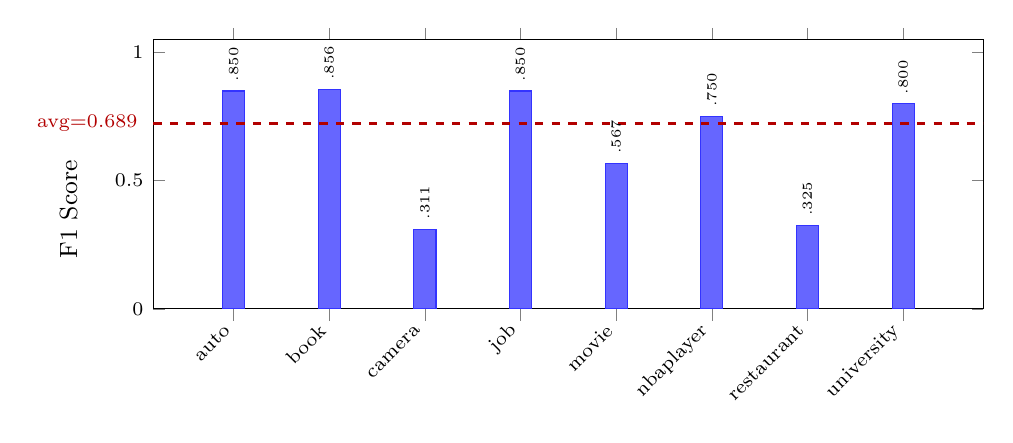
\begin{tikzpicture}
\begin{axis}[
  ybar,
  width=\columnwidth,
  height=5cm,
  bar width=8pt,
  ymin=0, ymax=1.05,
  ylabel={F1 Score},
  symbolic x coords={auto,book,camera,job,movie,nbaplayer,restaurant,university},
  xtick=data,
  x tick label style={rotate=45, anchor=east, font=\scriptsize},
  y tick label style={font=\scriptsize},
  ylabel style={font=\small, at={(axis description cs:-0.08,0.37)}},
  nodes near coords,
  every node near coord/.append style={font=\tiny, rotate=90, anchor=west},
  nodes near coords align={vertical},
  point meta=explicit symbolic,
  clip=false,
  enlarge x limits=0.12,
]
\addplot[fill=blue!60, draw=blue!80] coordinates {
  (auto,0.850) [.850]
  (book,0.856) [.856]
  (camera,0.311) [.311]
  (job,0.850) [.850]
  (movie,0.567) [.567]
  (nbaplayer,0.750) [.750]
  (restaurant,0.325) [.325]
  (university,0.800) [.800]
};
% Average line
\draw[dashed, thick, red!70!black] (rel axis cs:0,0.689) -- (rel axis cs:1,0.689)
  node[pos=0, anchor=east, font=\scriptsize, xshift=-2pt] {avg=0.689};
\end{axis}
\end{tikzpicture}
\caption{SWDEベンチマーク: バーティカル別F1スコア(検出フィールド)}
\ecaption{SWDE benchmark: F1 scores by vertical (found fields).}
\label{fig:swde}
\end{figure}


XPathが正常に生成されたフィールドではF1=0.689を達成し,
検出フィールドの60\%がF1=1.0(完全抽出)であった.
未検出フィールドを含む厳密F1は0.317である.

AXE\cite{axe2026}はラベル付き訓練データを用いた教師あり設定でF1 88.1\%を報告しているが,
XPathGenieはゼロショット(訓練データなし)での評価であり,両者の条件は本質的に異なる.
厳密F1=0.317との差は主に以下の3要因に起因する:
(1) \textbf{フィールド発見カバレッジ}——XPathGenieは対象87フィールド中29フィールド(46\%)
のみを検出した.これは抽出精度ではなくフィールド発見の問題であり,
検出されたフィールドの60\%がF1=1.0(完全抽出)を達成している.
(2) \textbf{アーキテクチャのスコープ不一致}——圧縮パイプラインが\texttt{<head>}を除外するため,
\texttt{<title>}タグからの抽出を試みない.
(3) \textbf{サイトレベルの失敗}——22サイト中5サイトがフィールドゼロを返した
(レガシーHTML構造による圧縮限界).

自動セマンティック評価(SWDEの400フィールド-値ペア)では
意味的精度78.0\%を達成し,手動評価の95.0\%を補完する結果となった.

%% --- 4.3 ---
\subsection{クロスドメイン・多言語評価}

医療求人以外の日本語7サイト(EC,不動産,レシピ,飲食店,ニュース)で
マクロ平均ヒット率79.4\%を達成した(SUUMO,Cookpadが100\%).
英語10サイト・10ドメイン(各3ページ,計30ページ)の評価では,
成功7サイトでマクロ平均ヒット率78.7\%であり,
GitHubおよびQuotes to Scrapeで100\%,StackOverflow 86\%,PyPI 80\%に達した.

いずれの評価でも一貫したパターンが確認された:
セマンティックなHTML構造(th/td,dt/dd,BEM\footnote{Block Element Modifier:CSSクラス名の命名規則の一つ.}命名規則のclass名)を持つサイトでは
ドメインに依存せず高精度を達成し,
CSS-in-JSフレームワーク(styled-components等)やSPAサイトでは性能が低下する.
この結果は\textbf{半構造化コンテンツ仮説}——XPathGenieはセマンティックなHTML構造を
持つコンテンツ指向ページにおいてドメイン非依存で有効であり,
失敗事例はアルゴリズムの欠陥ではなく構造的前提の違反を反映する——を支持する.

\subsection{失敗事例の分析}

体系的な失敗モードとして以下の4パターンが特定された:
(1) \texttt{text()=}述語における空白不一致(圧縮-生成ギャップ),
(2) CSSフレームワークのラッパーdivによるDOM深度の不一致,
(3) 非標準的なラベルテキストの変異(例:「お給料」vs「給与」),
(4) 特定求人種別にのみ存在する条件付きコンテンツ.
HTML構造別では,th/tdテーブル(87.1\%),dt/dd定義リスト(88.9\%),
混在構造(96.2\%)が高精度であるのに対し,
div/span(Tailwind等)は23.6\%と大幅に低下した.

\subsection{アブレーション研究}

代表5サイトで4条件のアブレーションを実施した:
フルパイプライン(88.1\%),圧縮なし(65.0\%,$-$23.1pp),
精緻化なし(88.8\%,+0.7pp),normalize-spaceなし(82.9\%,$-$5.2pp).
HTML圧縮が最も重要な構成要素であり,圧縮なしでは2サイトがJSONパースエラーとなった.
\texttt{normalize-space()}の効果は空白の多いHTMLを持つサイトに集中する
(caresta: 81.5\% $\to$ 46.2\%).

%% =============================================
\section{設計原則}

\textbf{「AI Once, DOM Forever」——コスト最適化:}
XPathGenieの最も重要なアーキテクチャ上の決定は,LLMの呼び出しをサイトマッピング
ごとに正確に1回(AI精緻化が発動する場合は2回)に限定することである.
ここで「Once」とは実行時(クローリング時)にAIが不要であることを意味し,
初期構築時の精緻化段階でAI再推論(Tier 2)が発動する場合でも
構築フェーズに限定される.
その出力は再利用可能なXPath式の集合であり,決定論的でポータブルかつ
AIインフラなしで実行可能である.
$n$ページのサイトに対し,ページ単位LLM抽出はページ数に比例する$O(n)$のAIコストを
要するが,XPathGenieはページ数に依存しない$O(1)$のAIコスト(一度限りの生成)+
$O(n)$の決定論的DOMクエリである.
10,000ページでもAIコストは1ページと同一である.
二段階精緻化はさらにコストを最適化する.Tier 1の機械的絞り込みはDOM走査により
大半の複数マッチケースを解決し(AIコストゼロ),より高コストなAI再推論は
値の曖昧性解消が真に必要なケースにのみ留保される.

圧縮パイプラインは\texttt{<head>}メタデータを除外し\texttt{<body>}コンテンツのみを
対象とする.これは本番クローリングの要件に基づく意図的なトレードオフである.
定期クローリングでは投稿日等の時間的メタデータはクローラ自身の観測スケジュールから
導出されるのが一般的であり,\texttt{<title>}タグよりもページ本文から抽出された
タイトルが好まれる.HTML圧縮はLLMのトークン消費に直接影響するため,
クローリングインフラで既に利用可能なメタデータを除外することで
分析あたりの不要なトークン支出を回避している.

\textbf{役割の逆転:}
従来のWebスクレイピングでは人間がXPathを記述し(創造的だが誤りを生じやすい),
機械がそれを実行する(機械的かつ信頼性が高い)という分業であった.
XPathGenieではこの役割が逆転する:機械がXPathを記述し(LLM推論+機械的絞り込み),
人間がXPathを検証する(Aladdinによる抽出値の目視確認).
一方が作成し他方が検証するという構造的関係は維持しつつ,各エージェントの
認知的強みに応じた配置となる.人間は文脈に即した品質判断に長けているが,
\texttt{//dl[dt[normalize-space()='給与']]/dd}をゼロから構築することは得意ではない.
Jasmineのセクション選択も同じ原則の適用であり,人間のタスクは構築(XPathの記述,
ルールの実装)から認識(値の検証,関連コンテンツの認識)へと移行している.

\textbf{Why $>$ What——LLMへの意図の伝達:}
プロンプト設計における中核的原則は,制約が何であるかを示すだけでなく,
なぜその制約が必要かをLLMに伝えることである.
例えば\texttt{contains(@class,...)}の使用指示に
「クラス属性は複数の値を持つことが多いため」と理由を併記する.
Want Listモードの意味的記述も同じ原則の適用であり,
例えば\texttt{"contract": "雇用形態 (employment type)"}という記述により
LLMは「雇用形態」「就業形態」「Employment Type」等の異なるラベルを
同一フィールドに対応付けることが可能となる.
機械的絞り込みにおける中間コンテナの自動検出も同じ原則の発現であり,
コンテナのクラス名をハードコーディングするのではなく祖先チェーンを走査して
動的に発見することで,サイト固有の設定なしに任意のサイト構造に適応する.

%% =============================================
\section{制限事項と今後の課題}

\textbf{SPA対応:}
XPathGenieは現在HTTPリクエストによる生HTML取得に依存している.
JavaScriptでコンテンツを動的にレンダリングするサイト(React, Vue, Angular
によるSPA)では,空またはスケルトンのHTMLが返されるためXPath生成が不可能となる.
評価対象35サイト中7サイトがSPAであり除外された.
ヘッドレスブラウザ(例:Playwright)を利用したJavaScriptレンダリング後の
HTML取得は今後の拡張として計画している.

\textbf{CSSフレームワーク互換性:}
ユーティリティクラス型フレームワーク(Tailwind CSS等)では意味的情報が
非記述的なクラス名(\texttt{w-11/12}, \texttt{flex}等)を持つ深くネストされた
要素にエンコードされるため精度が低下する.
CSS-in-JS(styled-components等)はさらに根本的な課題を呈し,
クラス名がビルド時のハッシュ値でデプロイごとに変化するため
安定した構造的アンカーが存在しない.
Yahoo! News(styled-components)のヒット率は14\%であった一方,
Cookpad(TailwindだがセマンティックなHTML併用)は100\%を達成しており,
制限要因はユーティリティクラスそのものではなくDOM階層における意味的構造の有無である.

\textbf{圧縮-生成ギャップ:}
HTML圧縮パイプラインは空白の正規化やテキストの切り詰めを行うため,
LLMが参照する圧縮HTMLと生成されたXPathが評価される生HTMLの間に構造的乖離が生じる.
例えば\texttt{<td>\textbackslash n~~~~勤務地\textbackslash n~~</td>}は
\texttt{<td>勤務地</td>}に圧縮され,\texttt{text()='勤務地'}は圧縮HTMLでは
成功するが生HTMLでは失敗する.\texttt{normalize-space()}の採用により
空白に起因するケースは緩和される.
圧縮器が誤ったコンテンツ領域を選択するセクション選択エラーについては,
Jasmineが人間介入のエスケープ手段を提供する.

\textbf{サイト構造の変化:}
生成されたXPathは分析時点のDOM構造に本質的に依存する.
サイトのリデザインによりXPathが無効となる可能性があり,
定期的な再分析メカニズムや変更検知システムの導入が望まれる.

\textbf{モデル依存性:}
全評価はGemini 2.5 Flash\cite{gemini2025}で実施した.
構造化プロンプティングとJSONモード出力に依拠しており
他モデルへの移植可能性が示唆されるが,実証的には未検証である.
より小規模なモデルでは性能が異なる可能性がある.

\textbf{再現性:}
主要23サイトのHTMLスナップショットは未アーカイブであるが,
SWDEおよび英語評価では全ページをアーカイブし再現可能性を確保した.
LLMの非決定性(\texttt{temperature=0.1}にもかかわらず)により実行間で
軽微な変動が生じうる.21サイト・3回実行の再現性調査では,
8サイトがSD=0の完全安定,全体平均ヒット率83.1\%であった.
2サイト(phget, MRT-nurse)は0\%--100\%の極端な分散を示し,
非標準的なHTML構造(div/spanレイアウト)と相関していた.

%% =============================================
\section{結論}

XPathGenieは,HTML圧縮(97\%削減),LLM推論,マルチページ検証,
二段階精緻化を統合し,セマンティックなHTML構造を持つ本番Webサイトにおいて
高い抽出精度を達成した.
23サイトの手動評価でセマンティック精度95.0\%(100サンプル),
SWDEベンチマーク(22サイト)では検出フィールドF1=0.689を達成した.
厳密F1=0.317との差は主にフィールド発見カバレッジ(46\%)に起因し,
検出フィールドの60\%がF1=1.0(完全抽出)であることから
コア抽出メカニズムは健全である.
フィールド発見の改善(圧縮とプロンプティングの強化)が
最もレバレッジの高い改善機会である.

圧縮-生成ギャップから重要なエンジニアリング上の知見が得られた.
HTML圧縮器が空白を正規化するため\texttt{text()=}述語が検証時に失敗するが,
\texttt{normalize-space()}の採用により解消され,
空白の多いサイトの精度が劇的に向上した(例:ph-10: 0\% $\to$ 90.8\%).
この問題は,LLM推論の前に入力の表層形式を変換するあらゆるシステムにおいて
推論時の表現と実行時の環境との間に意味的整合性のリスクをもたらすという
一般的原則を例示している.

「AI Once, DOM Forever」の設計により,初期生成後の運用コストはゼロとなる.
$n$ページのサイトに対し,ページ単位LLM抽出のページ数比例コストに対して
XPathGenieは一定のAIコスト+決定論的DOMクエリのみで動作する.
実際のサイトあたりのエンドツーエンド所要時間は,自動生成(約20秒)と
Aladdinによる人間の検証(5--15分)を含めて約20分であり,
手作業によるXPath記述に通常要する5--6時間と比較して大幅に短縮されている.
Genie--Jasmine--Aladdinの3ツール構成は,
機械が作成し人間が検証するという完全なワークフローを確立し,
Web データ抽出における従来の分業を逆転させた.

今後の課題として,フィールド発見カバレッジの改善(圧縮とプロンプティングの強化),
SPA対応のためのヘッドレスブラウザ統合,
および他のLLMモデルでの性能検証が挙げられる.
XPathGenieは,LLMの推論能力を一度限りの知識抽出に集中させ,
その成果を決定論的に再利用可能な形式に変換するという設計パラダイムを示した.
このアプローチはWebデータ抽出に限らず,
LLMの出力を永続的なルールとして定着させる応用全般に適用可能であると考える.

\begin{acknowledgment}
AIアシスタント テディ(Claude, Anthropic)による開発支援・文書作成支援に感謝する.
\end{acknowledgment}

\begin{thebibliography}{99}

\bibitem{kushmerick1997}
Kushmerick, N., Weld, D.\,S. and Doorenbos, R.:
Wrapper Induction for Information Extraction,
{\it Proc.\ IJCAI}, pp.\,729--735 (1997).

\bibitem{dalvi2011}
Dalvi, N., Kumar, R. and Soliman, M.:
Automatic Wrappers for Large Scale Web Extraction,
{\it Proc.\ VLDB Endowment}, Vol.\,4, No.\,4, pp.\,219--230 (2011).

\bibitem{kohlschutter2010}
Kohlsch\"{u}tter, C., Fankhauser, P. and Nejdl, W.:
Boilerplate Detection Using Shallow Text Features,
{\it Proc.\ WSDM}, pp.\,441--450 (2010).

\bibitem{lockard2020}
Lockard, C., Dong, X.\,L., Einolghozati, A. and Shiralkar, P.:
ZeroShotCeres: Zero-Shot Relation Extraction from Semi-Structured Webpages,
{\it Proc.\ ACL}, pp.\,8105--8117 (2020).

\bibitem{li2022}
Li, J., Xu, Y., Cui, L. and Wei, F.:
MarkupLM: Pre-Training of Text and Markup Language for Visually Rich Document Understanding,
{\it Proc.\ ACL}, pp.\,6078--6087 (2022).

\bibitem{deng2022}
Deng, X., Sun, Y., Galley, M. and Gao, J.:
DOM-LM: Learning Generalizable Representations for HTML Documents,
{\it arXiv:2201.10608} (2022).

\bibitem{perini2024}
Perini, M., Samardzic, L. and Pozzoli, M.:
ScrapeGraphAI: A Web Scraping Python Library That Uses LLM and Direct Graph Logic,
{\it arXiv:2411.13104} (2024).

\bibitem{xpathagent2024}
XPath Agent:
Multi-Sample XPath Generation via Two-Stage LLM Pipeline,
{\it arXiv:2502.15688} (2024).

\bibitem{axe2026}
AXE: Adaptive X-Path Extractor:
DOM Pruning for Efficient LLM-Based XPath Extraction with Grounded Resolution,
{\it arXiv:2602.01838} (2026).

\bibitem{hao2011}
Hao, Q., Cai, R., Pang, Y. and Zhang, L.:
From One Tree to a Forest: A Unified Solution for Structured Web Data Extraction,
{\it Proc.\ SIGIR}, pp.\,775--784 (2011).

\bibitem{gemini2025}
Google:
Gemini 2.5 Flash,
{\it Google DeepMind} (2025).
\url{https://deepmind.google/technologies/gemini/}

\bibitem{ferrara2014}
Ferrara, E., De Meo, P., Fiumara, G. and Baumgartner, R.:
Web Data Extraction, Applications and Techniques: A Survey,
{\it Knowledge-Based Systems}, Vol.\,70, pp.\,301--323 (2014).

\end{thebibliography}

\end{document}
